\chapter{Introducción general}
\label{ch:introduccion}

Este capítulo presenta de forma breve el contexto del trabajo realizado.
Se explica la problemática solucionada y los conceptos necesarios para la lectura de la memoria.

\newcommand{\keyword}[1]{\textbf{#1}}
\newcommand{\tabhead}[1]{\textbf{#1}}
\newcommand{\code}[1]{\texttt{#1}}
\newcommand{\file}[1]{\texttt{\bfseries#1}}
\newcommand{\option}[1]{\texttt{\itshape#1}}
\newcommand{\grados}{$^{\circ}$}

\section{El espacio como recurso estratégico}
\label{sec:1space}

El espacio exterior es un recurso estratégico para el bienestar de la humanidad.
Dado que, su explotación permite mejorar la producción de bienes y servicios.
Además, provee datos de valor científico que incrementan la calidad de vida de las personas \citep{BOOK:spaceage}.

El marco jurídico que regula la explotación del recurso es el Tratado sobre el espacio exterior de 1967.
Del cual, la República Argentina es miembro desde el 27 de enero de ese año.
Los países pueden reclamar cualquiera de las órbitas disponibles pero tienen la obligación de hacer uso dentro de un margen de tiempo determinado.
Luego, si el país no ocupó la órbita pierde el derecho a usarla \citep{BOOK:resurrect}.

El mercado de la explotación espacial está compuesto de estados y empresas.
Siendo las últimas quienes adquirieron el protagonismo en el siglo XXI \citep{ARTICLE:transition}.
El marco jurídico y la competencia en este rubro empuja a las compañías a innovar de forma permanente.
En particular, con nuevas técnicas y tecnologías que permitan abaratar el costo de las misiones.

El cliente de este trabajo es INVAP S.E. y es una empresa de la provincia de Río Negro.
La compañía es modelo en su tipo y realiza proyectos tecnológicos complejos en áreas como: reactores nucleares, satélites y radares.
En la figura \ref{fig:saocom} se puede observar un satélite realizado por la empresa.

\newpage

\begin{figure}[htbp]
	\centering
	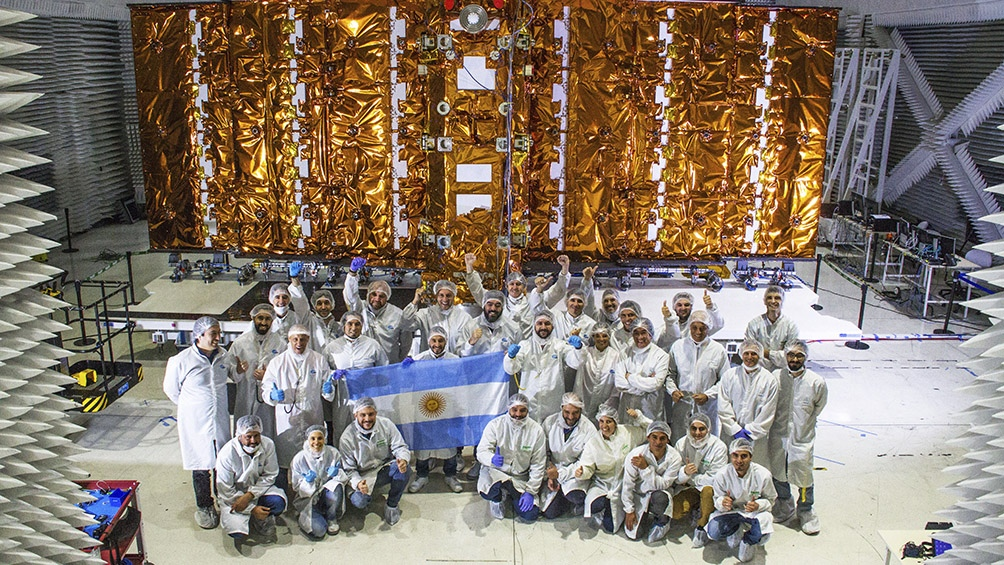
\includegraphics[width=\textwidth]{./Figures/invapsaocom.jpg}
	\caption{Satélite SAOCOM\protect\footnotemark.}
	\label{fig:saocom}
\end{figure}

\footnotetext{Imagen tomada de la página oficial de INVAP S.E. \citep{WEBSITE:invap}}

\section{Radiación cósmica y sus efectos}
\label{sec:radiacion}

El sol produce partículas de luz e iones pesados que de forma conjunta se denominan viento solar.
Este fenómeno es atenuado antes de llegar a la superficie del planeta gracias al campo magnético terrestre \citep{WEBSITE:structure_space_radiation}.
Como se puede ver en la figura \ref{fig:viento}, las partículas son desviadas por el campo.
Luego, este queda deformado por el viento solar y se genera una magnetosfera asimétrica.
En la tabla \ref{tab:capasmagneticas} se puede observar las características de la asimétria.

\begin{table}[h]
	\centering
	\caption[Cinturón de Van Allen]{Cinturón de Van Allen \citep{WEBSITE:structure_space_radiation}.}
	\begin{tabular}{l c c}    
		\toprule
		\textbf{Cinturon} & \textbf{Frontera}           & \textbf{Partícula dominante}\\
		\midrule
		Interior          & 1,2 - 2,5 radios terrestres & Protones de alta energía\\		
		Exterior          & 2,8 - 12 radios terrestres  & Electrones de alta energía\\
		\bottomrule
		\hline
	\end{tabular}
	\label{tab:capasmagneticas}
\end{table}

La electrónica de los satélites tiene un alto grado de exposición al viento solar.
Esto significa que la probabilidad de incidencia de una partícula cargada en el circuito es mayor.
La incidencia de una partícula genera una traza densa de pares electrón-hueco en los semiconductores \citep{ARTICLE:velazco}.
Además, es posible que esta ionización cause un pulso transitorio de corriente.
En la figura \ref{fig:bitflip} se puede ver el efecto de la radiación sobre los transistores de un integrado.

Los efectos de la radiación cósmica sobre el circuito pueden ser transitorios o permanentes.
Los permanentes se deben a la destrucción de una parte del circuito.
Esta destrucción es producto de: el disparo de componentes activos parásitos o la generación de plasma dentro del encapsulado \citep{WEBSITE:effects_on_devices}.
Finalmente, en la tabla \ref{tab:radiacion} se puede ver un resumen de los tipos de errores generados por la radiación cósmica.

\newpage

\vfill
\begin{figure}[htbp]
	\centering
	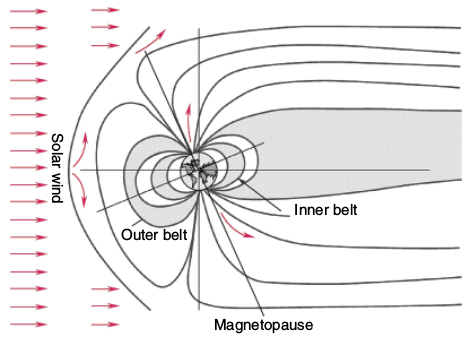
\includegraphics[width=0.8\textwidth]{./Figures/vientosolar.jpg}
    \caption{Capas magnéticas de la tierra y viento solar\protect\footnotemark.}
	\label{fig:viento}
\end{figure}

\footnotetext{Imagen tomada del artículo \emph{Structure of space radiation} \citep{WEBSITE:structure_space_radiation}}

\vfill

\begin{figure}[htbp]
	\centering
	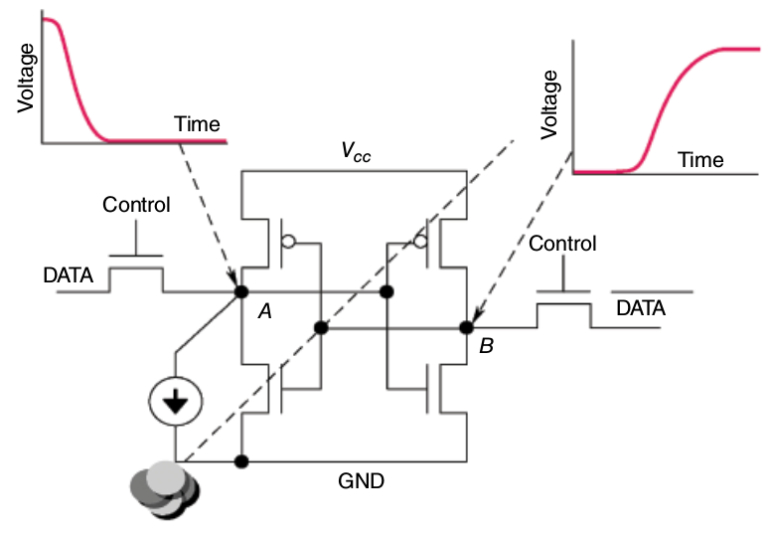
\includegraphics[width=0.8\textwidth]{./Figures/bitflip.jpg}
    \caption{Ejemplo simplificado de \emph{bit flip} en un bloque \emph{SDRAM}\protect\footnotemark.}
	\label{fig:bitflip}
\end{figure}

\footnotetext{Imagen tomada del artículo \emph{Effects of space radiation on electronic devices} \citep{WEBSITE:effects_on_devices}}

\vfill

\begin{table}[h]
	\centering
	\caption[Efectos de la radiación cósmica]{Efectos producidos por la radiación cósmica \citep{WEBSITE:structure_space_radiation}.}
	\begin{tabular}{l c c}    
		\toprule
		\textbf{Evento}      & \textbf{Acrónimo} & \textbf{Efecto}\\
		\midrule
		Latch-up             & SEL               & Pico de corriente\\		
		Upset                & SEU               & Alteración de datos\\
		Funtional Interrupt  & SEFI              & Cambios en la configuración\\
		Transient            & SET               & Pico de tensión\\
		Burnout              & SEB               & Activación de transistores parásitos\\
		Gate Rapture         & SEGR              & Generación de plasma de alta densidad\\
		\bottomrule
		\hline
	\end{tabular}
	\label{tab:radiacion}
\end{table}

\newpage

\section{Calificación espacial e iniciativa \emph{new space}}
\label{sec:newspace}

A los efectos vistos en la sección \ref{sec:radiacion} se suman: el estrés mecánico del lanzamiento y los cambios de temperatura en la órbita.
Este ambiente genera la necesidad de utilizar componentes con calificación espacial.
Para que un componente alcance la calificación espacial se debe someter a un largo y costoso proceso de acreditación.
Luego, estos componentes adolecen de un elevado precio y atraso tecnológico frente a los del mercado masivo \citep{ARTICLE:negocio}.

La irrupción del sector privado vista en la sección \ref{sec:1space}, trajo una nueva iniciativa comercial denominada \emph{new space}.
Esta iniciativa busca bajar los costos al utilizar componentes no calificados para su uso espacial.
Además, existe la ventaja adicional de introducir tecnología de vanguardia.


El caso de \emph{Starlink} es un ejemplo de \emph{new space} particular.
Su volumen de satélites lanzados permite realizar conclusiones estadísticas significativas.
En particular, su poca capacidad para cumplir sus objetivos si se mantiene la actual tasa de mortalidad de sus satélites \citep{ARTICLE:cibils}.
En las figura \ref{fig:starlinkdeath} se puede observar que la constelación no logrará alcanzar la población deseada.
 
Al problema de población de \emph{Starlink} se suma la gran cantidad de polución generada.
Los satélites fuera de servicio no pueden ser desorbitados y persisten en forma de \emph{debris}.
Como se puede ver en la tabla \ref{tab:starlinkdebris}, el volumen de basura generado es significativo.

\begin{table}[h]
	\centering
    \caption[Proyección de \emph{debris}]{Proyección de \emph{debris} de \emph{Starlink} \citep{ARTICLE:cibils}.}
	\begin{tabular}{c c c c c}    
		\toprule
        \textbf{Lanzamientos} & \textbf{Satélites} & \textbf{Total lanzados} & \textbf{Población} & \textbf{Debris}\\
		\midrule
        12                    & 60                 & 7200                    & 2704               & 4046\\		
        12                    & 180                & 21600                   & 8105               & 12146\\		
        12                    & 400                & 48000                   & 18007              & 26994\\		
        180                   & 60                 & 108000                  & 40000              & 61200\\		
        60                    & 180                & 108000                  & 40000              & 61200\\		
        27                    & 400                & 108000                  & 40000              & 61200\\		
		\bottomrule
		\hline
	\end{tabular}
	\label{tab:starlinkdebris}
\end{table}

\newpage

\begin{figure}[htbp]
	\centering
    \begin{subfigure}{0.8\textwidth}
        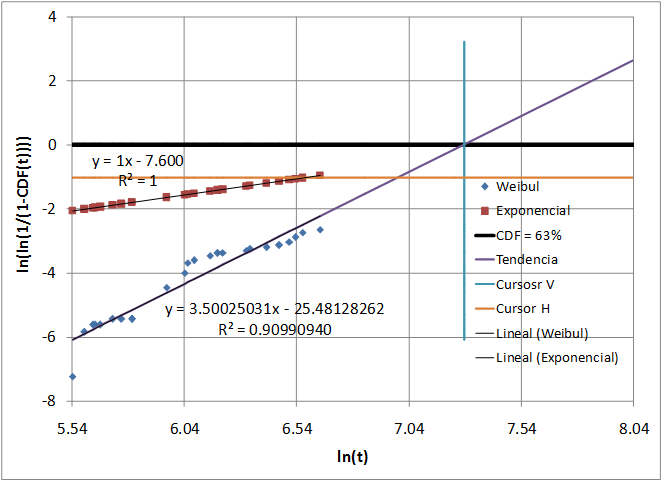
\includegraphics[width=\textwidth]{./Figures/starlinkdeath.png}
        \caption{Gráfico Weibull de expectativa de vida \emph{Starlink}.}
        \label{fig:starlinkdeathA}
    \end{subfigure}
    \hfill
    \begin{subfigure}{0.8\textwidth}
        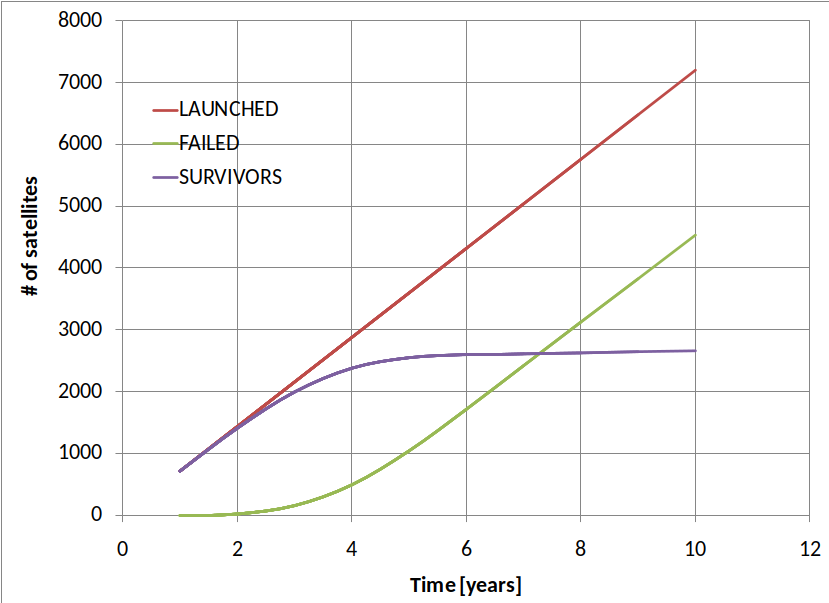
\includegraphics[width=\textwidth]{./Figures/starlinkpopulation.png}
        \caption{Proyección de la constelación \emph{Starlink}.}
        \label{fig:starlinkdeathB}
    \end{subfigure}
    \hfill
        \caption{Estadísticas de la constelación \emph{Starlink}\protect\footnotemark.}
        \label{fig:starlinkdeath}
\end{figure}
\footnotetext{Imagen tomada de la publicación de Roberto Cibils \citep{ARTICLE:cibils}.}

Las conclusiones del caso \emph{Starlink} muestran la importancia de tener herramientas para simular el ambiente espacial.
En particular, los efectos de la radiación cósmica para poder probar las técnicas de mitigación de errores seleccionadas.
Finalmente, este trabajo agrega valor al cliente al incrementar la confiabilidad de los satélites y evitar los problemas de la competencia.

\newpage

\section{Estado del arte}
\label{sec:arte}

Los ensayos de pruebas de radiación en tierra tienen las siguientes estrategias \citep{ARTICLE:velazco}:
\begin{itemize}
    \item Ensayo por \emph{software}: se introducen instrucciones espúreas en el código para generar errores.
    \item Ensayo por \emph{hardware}: se conecta un dispositivo que introduce errores durante la ejecución del programa.
    \item Ensayo por radiación: se introduce el dispositivo bajo prueba en una cámara de iones pesados como se puede ver en la figura \ref{fig:iones}.
\end{itemize}

\begin{figure}[htbp]
	\centering
	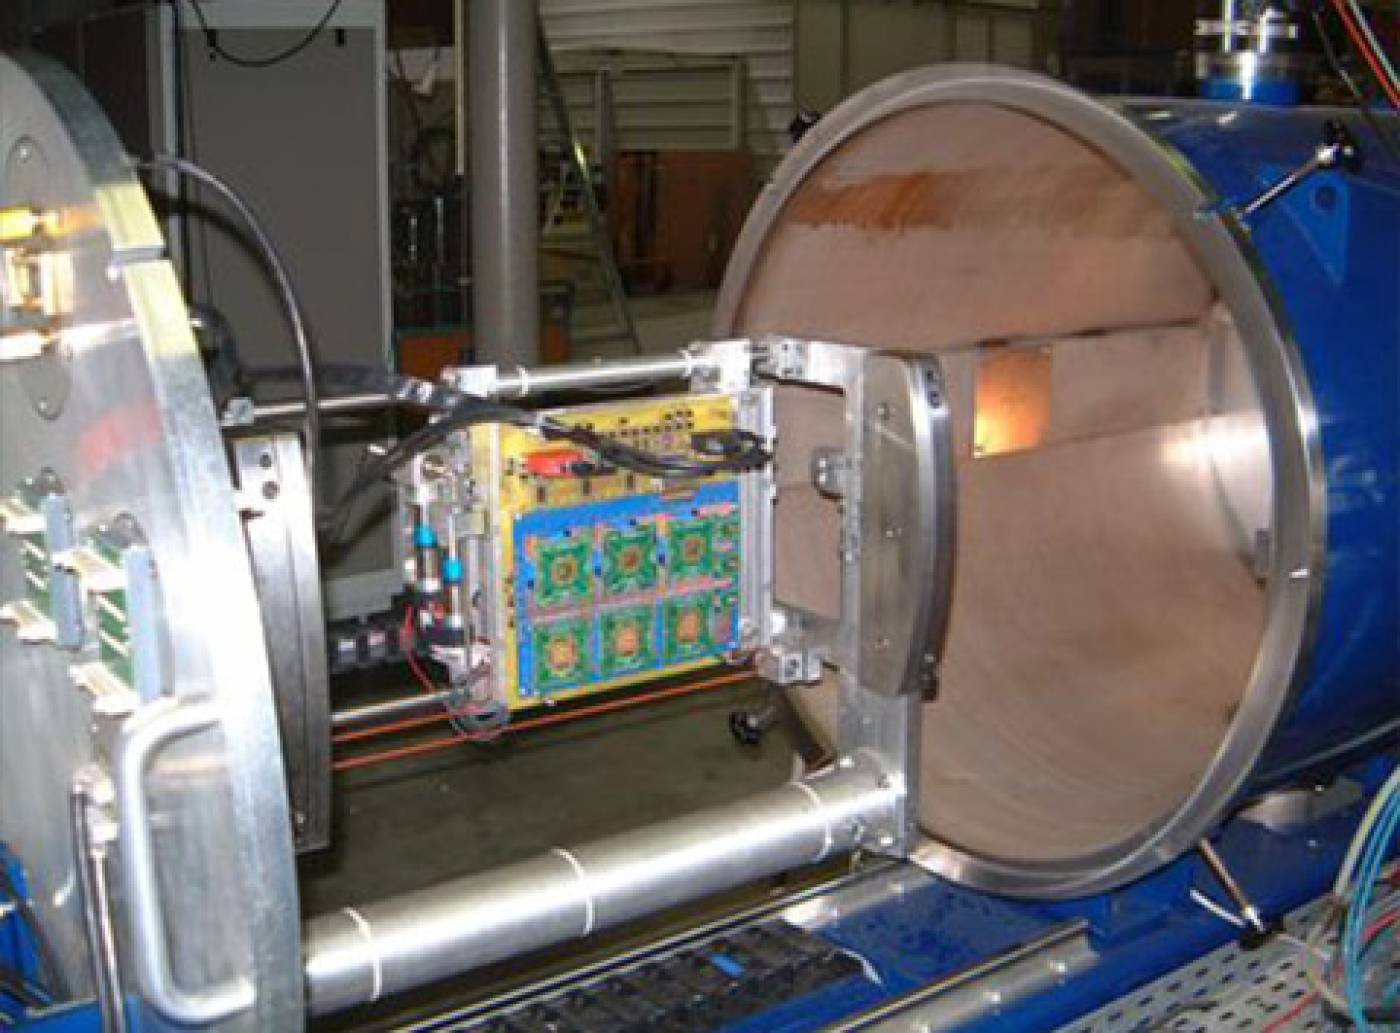
\includegraphics[width=\textwidth]{./Figures/heavy_ion_latchup_tests_in_louvain_la_neuve.jpg}
    \caption{Cámara de pruebas de iones pesados\protect\footnotemark.}
	\label{fig:iones}
\end{figure}

\footnotetext{Imagen tomada del sitio web ucl.ac.eu \citep{WEBSITE:heavy_ion}.}

Los métodos de ensayos mencionados presentan compromisos de diseño como se puede ver en la tabla \ref{tab:arte}.
El trabajo realizado es una solución del tipo ensayo por \emph{hardware}.

\begin{table}[h]
	\centering
	\caption[Comparación de métodos de simulación]{Comparación de métodos de simulación \citep{ARTICLE:velazco}.}
	\begin{tabular}{l c c c}    
		\toprule
        \textbf{Método}        & \textbf{Eficiencia} & \textbf{Costo} & \textbf{Limitación}\\
		\midrule
        \emph{Software}        & Baja                & Bajo           & Ciclos de CPU\\		
        \emph{Hardware}        & Media               & Medio          & Acceso al integrado\\
        Radiación              & Alta                & Alto           & Control del ensayo\\
		\bottomrule
		\hline
	\end{tabular}
	\label{tab:arte}
\end{table}

\section{Alcance del trabajo}
\label{sec:alcance}

El trabajo realizado se divide en dos partes:
\begin{enumerate}
    \item \emph{Firmware} para el dispositivo bajo prueba.
    \item Inyector de \emph{soft-errors} por consola de comandos.
\end{enumerate}

El \emph{firmware} en el dispositivo bajo prueba tiene la misión de validar su funcionamiento.
Esto se logró al verificar cada periférico de interés dentro del integrado.
Luego, se generan reportes periódicos que se envían al inyector por consola de comandos.
En la figura \ref{fig:dutsimple} se puede observar un diagrama en bloques simplificado.

\begin{figure}[htbp]
	\centering
	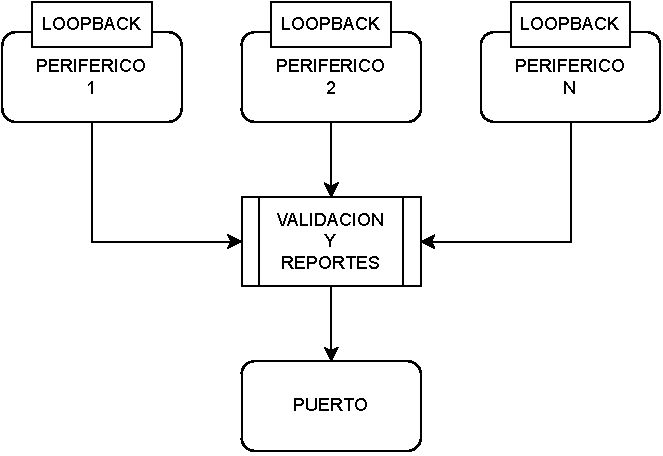
\includegraphics[width=0.7\textwidth]{./Figures/dutsimple.pdf}
    \caption{Diagrama simplificado del dispositivo bajo prueba.}
	\label{fig:dutsimple}
\end{figure}

El inyector por consola de comandos tiene la función de planificar los ensayos y gestionar la introducción de errores.
En la figura \ref{fig:sisesimple} se puede ver como interactúan las partes del sistema.

\begin{figure}[htbp]
	\centering
	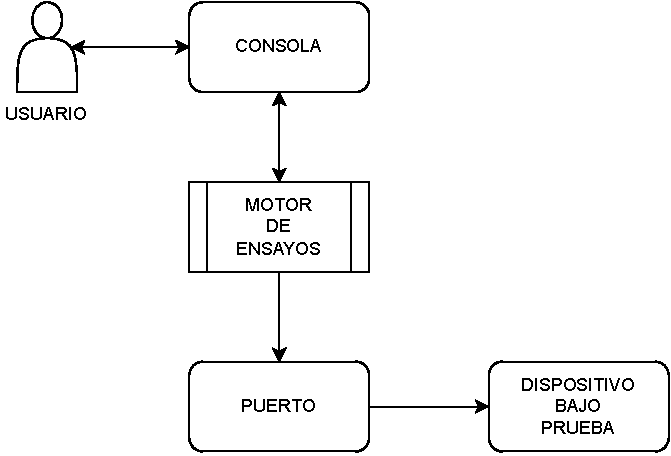
\includegraphics[width=0.7\textwidth]{./Figures/sisesimple.pdf}
    \caption{Diagrama simplificado del sistema de inyección de errores.}
	\label{fig:sisesimple}
\end{figure}

